% Options for packages loaded elsewhere
\PassOptionsToPackage{unicode}{hyperref}
\PassOptionsToPackage{hyphens}{url}
\documentclass[
  11pt,
  a4paper,
  fontset=none]{ctexart}
\usepackage{xcolor}
\usepackage[margin=22mm,headheight=15pt]{geometry}
\usepackage{amsmath,amssymb}
\setcounter{secnumdepth}{-\maxdimen} % remove section numbering
\usepackage{iftex}
\ifPDFTeX
  \usepackage[T1]{fontenc}
  \usepackage[utf8]{inputenc}
  \usepackage{textcomp} % provide euro and other symbols
\else % if luatex or xetex
  \usepackage{unicode-math} % this also loads fontspec
  \defaultfontfeatures{Scale=MatchLowercase}
  \defaultfontfeatures[\rmfamily]{Ligatures=TeX,Scale=1}
\fi
\usepackage{lmodern}
\ifPDFTeX\else
  % xetex/luatex font selection
\fi
% Use upquote if available, for straight quotes in verbatim environments
\IfFileExists{upquote.sty}{\usepackage{upquote}}{}
\IfFileExists{microtype.sty}{% use microtype if available
  \usepackage[]{microtype}
  \UseMicrotypeSet[protrusion]{basicmath} % disable protrusion for tt fonts
}{}
\makeatletter
\@ifundefined{KOMAClassName}{% if non-KOMA class
  \IfFileExists{parskip.sty}{%
    \usepackage{parskip}
  }{% else
    \setlength{\parindent}{0pt}
    \setlength{\parskip}{6pt plus 2pt minus 1pt}}
}{% if KOMA class
  \KOMAoptions{parskip=half}}
\makeatother
\usepackage{longtable,booktabs,array}
\usepackage{caption}
\captionsetup[table]{skip=6pt}
\newcounter{none} % for unnumbered tables
\usepackage{calc} % for calculating minipage widths
% Correct order of tables after \paragraph or \subparagraph
\usepackage{etoolbox}
\makeatletter
\patchcmd\longtable{\par}{\if@noskipsec\mbox{}\fi\par}{}{}
\makeatother
% Allow footnotes in longtable head/foot
\IfFileExists{footnotehyper.sty}{\usepackage{footnotehyper}}{\usepackage{footnote}}
\makesavenoteenv{longtable}
\usepackage{graphicx}
\makeatletter
\newsavebox\pandoc@box
\newcommand*\pandocbounded[1]{% scales image to fit in text height/width
  \sbox\pandoc@box{#1}%
  \Gscale@div\@tempa{\textheight}{\dimexpr\ht\pandoc@box+\dp\pandoc@box\relax}%
  \Gscale@div\@tempb{\linewidth}{\wd\pandoc@box}%
  \ifdim\@tempb\p@<\@tempa\p@\let\@tempa\@tempb\fi% select the smaller of both
  \ifdim\@tempa\p@<\p@\scalebox{\@tempa}{\usebox\pandoc@box}%
  \else\usebox{\pandoc@box}%
  \fi%
}
% Set default figure placement to htbp
\def\fps@figure{htbp}
\makeatother
\setlength{\emergencystretch}{3em} % prevent overfull lines
\providecommand{\tightlist}{%
  \setlength{\itemsep}{0pt}\setlength{\parskip}{0pt}}
% YOCO notes; style adapted from Attention/CN/pdf-header.tex.
\usepackage{fontspec}
\usepackage{enumitem}
\usepackage{fancyhdr}
\usepackage{fvextra}
\usepackage{etoolbox}
\usepackage{pdflscape}

\setmainfont[
  Path=/usr/local/texlive/2026/texmf-dist/fonts/opentype/public/tex-gyre/,
  UprightFont=texgyrepagella-regular.otf,
  BoldFont=texgyrepagella-bold.otf,
  ItalicFont=texgyrepagella-italic.otf,
  BoldItalicFont=texgyrepagella-bolditalic.otf
]{texgyrepagella-regular.otf}
\setsansfont[
  Path=/usr/local/texlive/2026/texmf-dist/fonts/opentype/public/tex-gyre/,
  UprightFont=texgyreheros-regular.otf,
  BoldFont=texgyreheros-bold.otf,
  ItalicFont=texgyreheros-italic.otf,
  BoldItalicFont=texgyreheros-bolditalic.otf
]{texgyreheros-regular.otf}
\setmonofont[
  Path=/usr/local/texlive/2026/texmf-dist/fonts/opentype/google/roboto/,
  UprightFont=RobotoMono-Regular.otf,
  BoldFont=RobotoMono-Bold.otf,
  ItalicFont=RobotoMono-Italic.otf,
  BoldItalicFont=RobotoMono-BoldItalic.otf,
  Scale=0.82
]{RobotoMono-Regular.otf}
\setCJKmainfont[
  Path=/System/Library/Fonts/Supplemental/,
  FontIndex=6,
  BoldFont=Songti.ttc,
  BoldFeatures={FontIndex=1}
]{Songti.ttc}
\setCJKsansfont[
  Path=/System/Library/Fonts/,
  FontIndex=1,
  BoldFont={STHeiti Medium.ttc},
  BoldFeatures={FontIndex=1}
]{STHeiti Light.ttc}
\setCJKmonofont[Path=/System/Library/Fonts/,FontIndex=1]{STHeiti Light.ttc}

\definecolor{attentionblue}{HTML}{174A7E}
\definecolor{attentiongray}{HTML}{5D6773}
\definecolor{attentionlink}{HTML}{1769AA}
\definecolor{codebg}{HTML}{F4F6F8}

\AtBeginDocument{%
  \hypersetup{
    linkcolor=attentionblue,
    urlcolor=attentionlink,
    citecolor=attentionblue,
    pdftitle={YOCO：跨层 KV 共享}
  }%
}

\ctexset{
  section={format=\LARGE\bfseries\sffamily\color{attentionblue},beforeskip=1.8ex,afterskip=1.2ex},
  subsection={format=\Large\bfseries\sffamily\color{attentionblue},beforeskip=1.6ex,afterskip=0.9ex},
  subsubsection={format=\large\bfseries\sffamily\color{attentiongray},beforeskip=1.4ex,afterskip=0.7ex}
}

\setlength{\parindent}{2em}
\setlength{\parskip}{0.35em}
\linespread{1.18}
\setlist{itemsep=0.25em,topsep=0.45em,leftmargin=2.4em}
\setcounter{tocdepth}{2}
\setcounter{secnumdepth}{0}

\pagestyle{fancy}
\fancyhf{}
\fancyhead[L]{\small\sffamily\color{attentiongray} YOCO}
\fancyhead[R]{\small\sffamily\color{attentiongray} Purshow’ Notes}
\fancyfoot[C]{\small\sffamily\thepage}
\renewcommand{\headrulewidth}{0.3pt}


\usepackage{caption}
\captionsetup{font=small,labelfont=bf}
\clearcaptionsetup{table} % Overview has no caption; clear Pandoc defaults.
\usepackage{float}
\floatplacement{figure}{H}
\AtBeginDocument{\renewcommand{\figurename}{图}}

% A single opening page: article title above an automatically linked contents.
\makeatletter
\renewcommand*\l@subsection{\@dottedtocline{2}{0em}{0em}}
\renewcommand*\l@subsubsection{\@dottedtocline{3}{1.6em}{0em}}
\makeatother
\newcommand{\NotesCover}[1]{%
  \pagenumbering{roman}%
  \thispagestyle{empty}%
  \vspace*{0mm}%
  {\centering
    \sffamily\bfseries\color{attentionblue}%
    \fontsize{26pt}{36pt}\selectfont #1\par
  }%
  \vspace{4mm}%
  {\color{attentionblue}\noindent\rule{\linewidth}{0.6pt}\par}%
  \vspace{4mm}%
  \begingroup
    \setlength{\parindent}{0pt}%
    \setlength{\parskip}{0.6em}%
    \tableofcontents
  \endgroup
}
\newcommand{\NotesCoverEnd}{%
  \clearpage
  \pagenumbering{arabic}%
}

% Compact wrapping overview table, following Attention and MoE notes.
\newcommand{\OverviewTableStyle}{%
  \fontsize{7.5pt}{8.8pt}\selectfont
  \setlength{\tabcolsep}{4pt}%
  \renewcommand{\arraystretch}{1.2}%
  \setlength{\extrarowheight}{6pt}%
  \setlength{\LTpre}{30pt}%
  \setlength{\LTpost}{0pt}%
  \setlength{\parskip}{0pt}%
}
\usepackage{bookmark}
\IfFileExists{xurl.sty}{\usepackage{xurl}}{} % add URL line breaks if available
\urlstyle{same}
% fallback for those not using the hyperref driver hyperxmp:
\makeatletter
\@ifundefined{xmpquote}{\newcommand{\xmpquote}[1]{#1}}{}
\makeatother
\hypersetup{
  hidelinks,
  pdfcreator={LaTeX via pandoc}}

\author{}
\date{}

\begin{document}

\NotesCover{YOCO：跨层 KV 共享}\NotesCoverEnd

随着 DeepSeek-V4.1-Flash 的发布，YOCO 也重新进入大众视野。在我看来，YOCO
是一篇非常优秀的工作，基于 YOCO，也出现了一些有趣的变种。

YOCO 的 motivation 主要有以下两点：

\begin{enumerate}
\def\labelenumi{\arabic{enumi}.}
\item
  \textbf{Prefill--Decode（PD）不对称。} Prefill 的主要工作是建立
  Cache，只有最后一个 Prompt token 负责产生第一次 logits，前面的 token
  都没有必要算 logits。普通 Transformer 因为每层都需要独立 KV
  Cache，很难充分利用这种不对称；而 YOCO 通过让后面的 Cross-Decoder
  共享同一份全局 Shared KV ，使长 Prefill的前面 token 在建立 Shared KV
  后即可提前退出，从而显著放大 PD
  不对称带来的收益。（此事在苏神的知乎亦有记载）
\item
  \textbf{从 Layer 维度压缩 KV Cache。} KV Cache 可以近似看成由
  entry（维度、头数）× sequence（长度）×
  layer（层数）三个维度共同决定。过去的工作已经从不同维度进行压缩：

  \begin{itemize}
  \tightlist
  \item
    \textbf{Entry}：GQA/MQA 减少 KV head 数，MLA 压缩单 token 的 KV
    表示维度 \(d_{\mathrm{KV}}\)。
  \item
    \textbf{Sequence}：CSA/HCA/Linear 等注意力减少对历史长度 \(N\)
    的缓存需求。
  \item
    \textbf{Layer}：YOCO 类的方法则从层数入手，让后面层共享同一份全局 KV
    Cache。
  \end{itemize}
\end{enumerate}

\subsection{一、YOCO}\label{ux4e00yoco}

\begin{center}

\pandocbounded{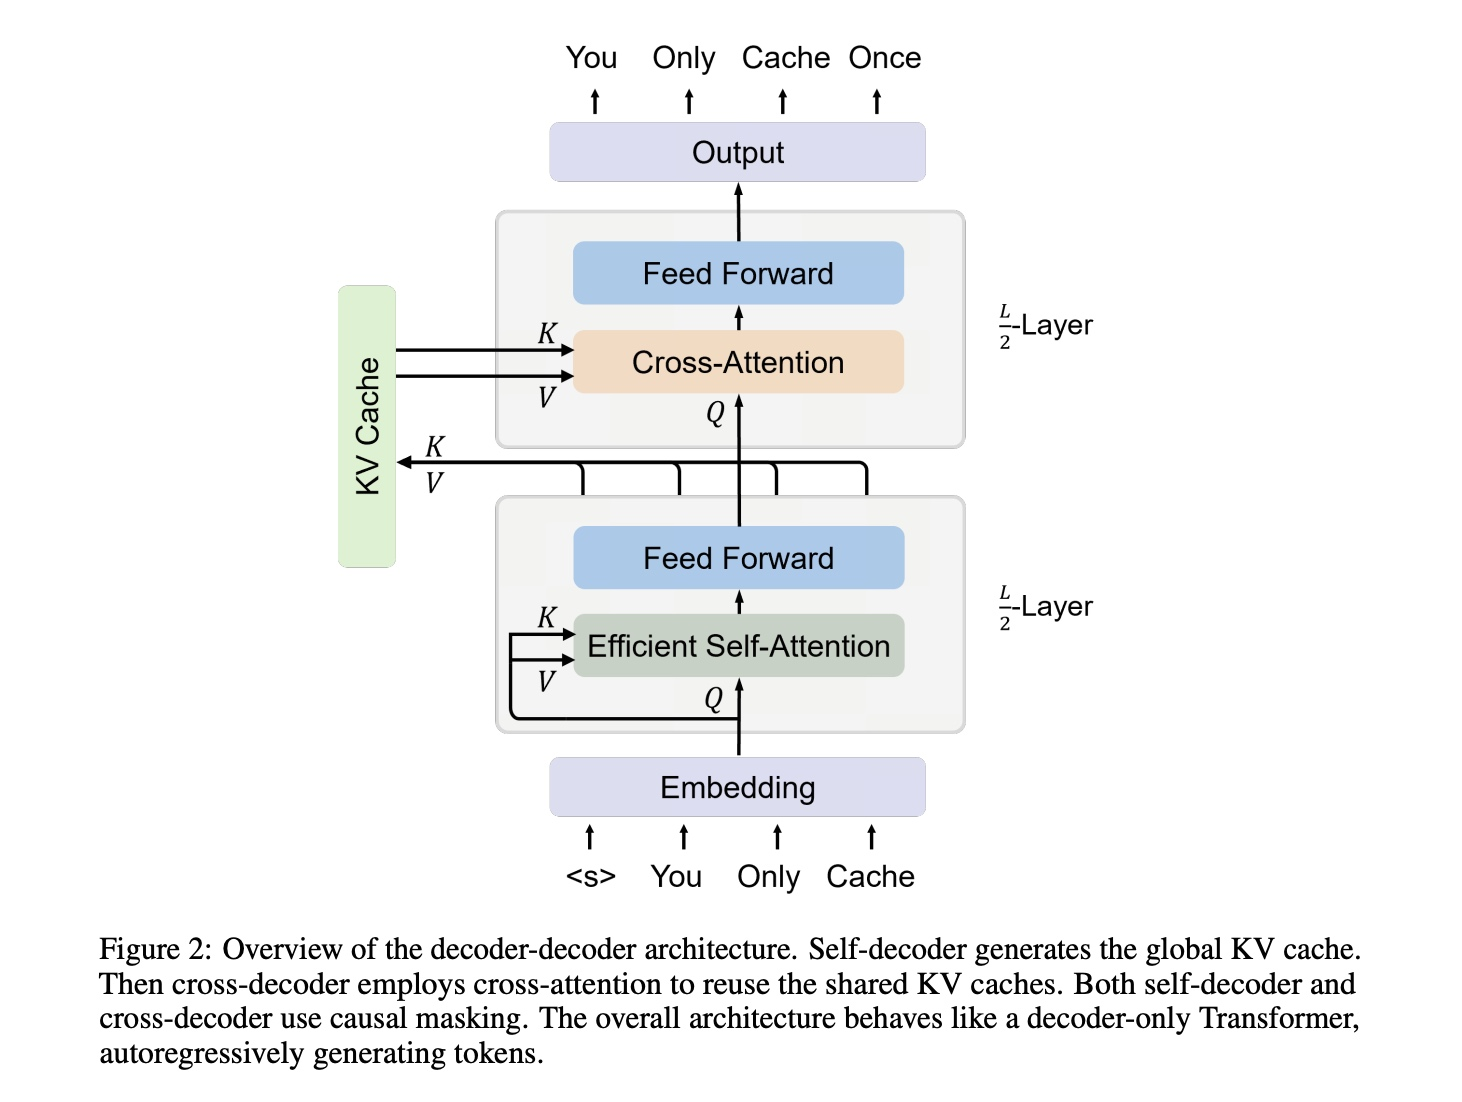
\includegraphics[keepaspectratio]{assets/YOCO_2.jpg}}

\end{center}

\begin{center}

\pandocbounded{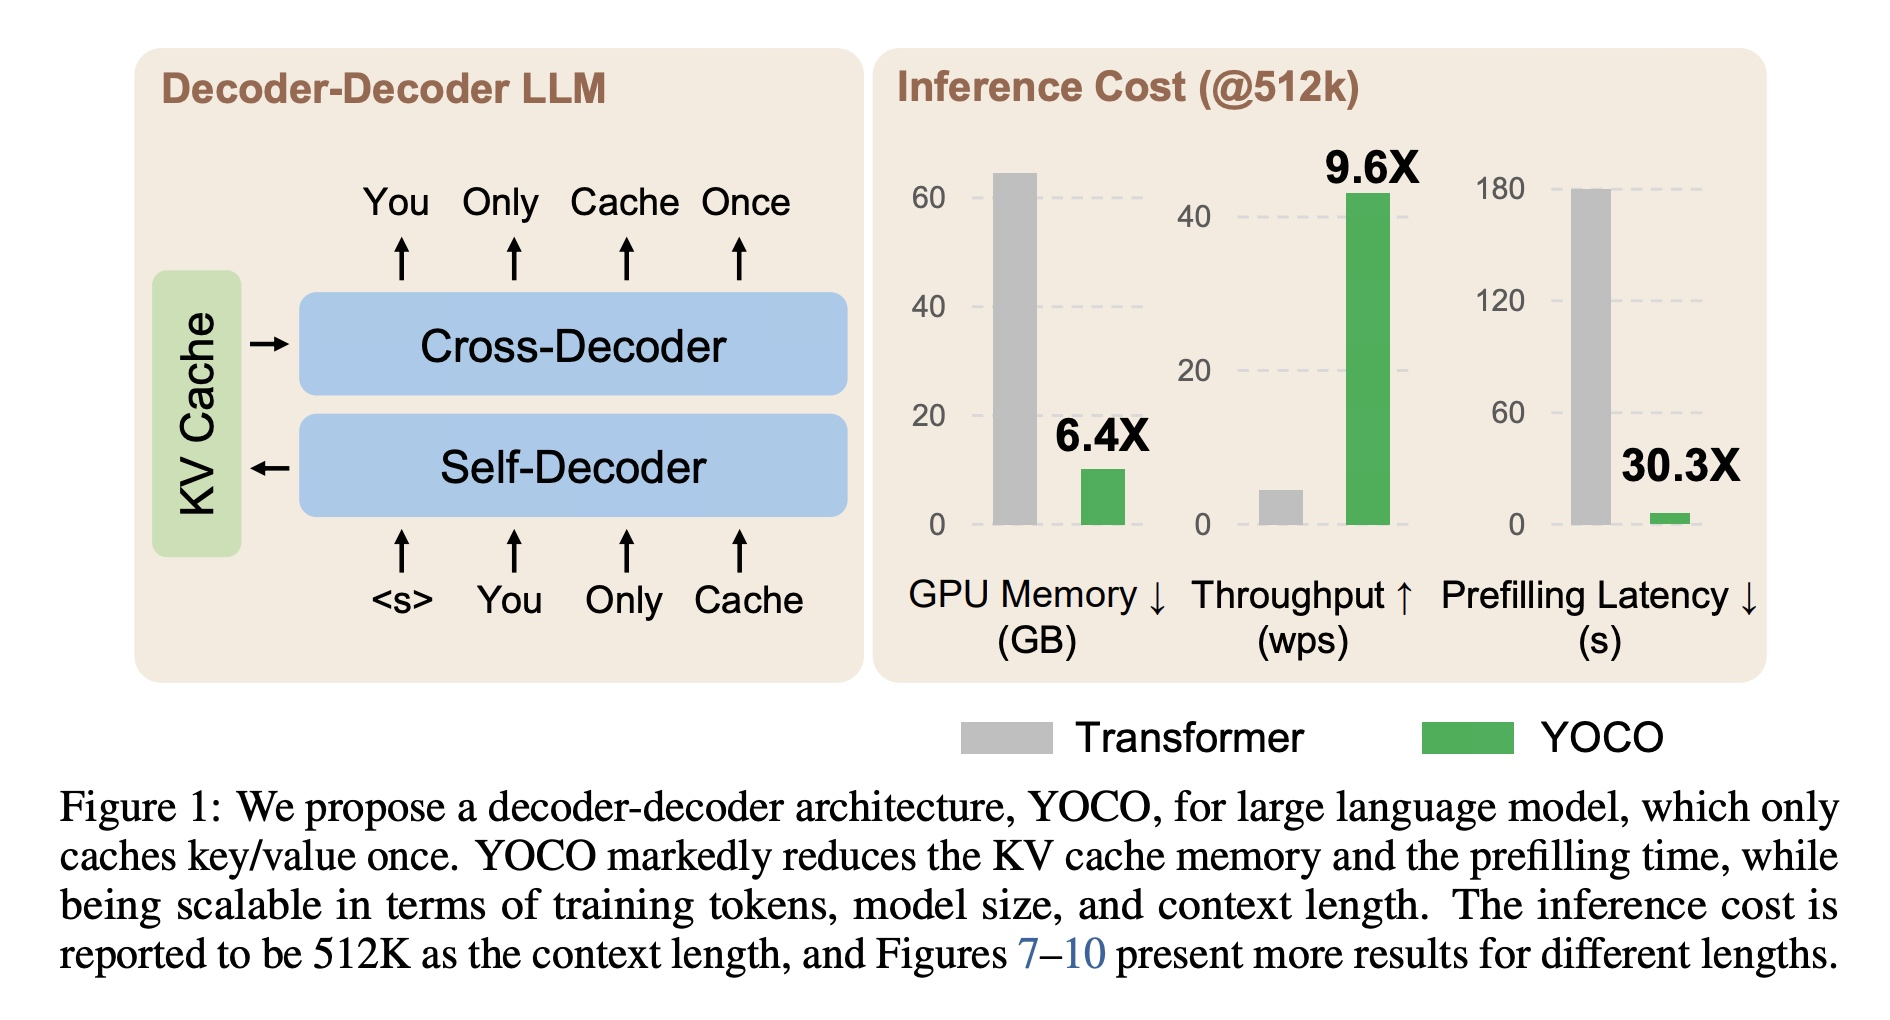
\includegraphics[keepaspectratio]{assets/YOCO_1.jpg}}

\end{center}

YOCO 的架构非常简单易懂：把标准 decoder-only Transformer
拆成上下两部分。

\textbf{前半部分是 Self-Decoder。} 激进一些的是，在这部分甚至采用了
gated retention 或 sliding-window
attention，进一步把整个上下文压成一份\textbf{共享的全局 KV Cache}。

\textbf{后半部分是 Cross-Decoder。} 每一层不再各自保存历史
K/V，而是用自己的 Query 去 cross-attend 同一份共享 KV。

标准 Transformer 的 KV Cache 从大致 \(O(LND)\) 降到：

\[
O\!\left((N+L)D\right).
\]

更妙的是，Prefill 阶段完全不需要跑后面的 Cross-Decoder（这在现在的 agent
场景的超长输入中，确实是太实用了）。

\subsection{二、YOCO-U}\label{ux4e8cyoco-u}

\begin{center}

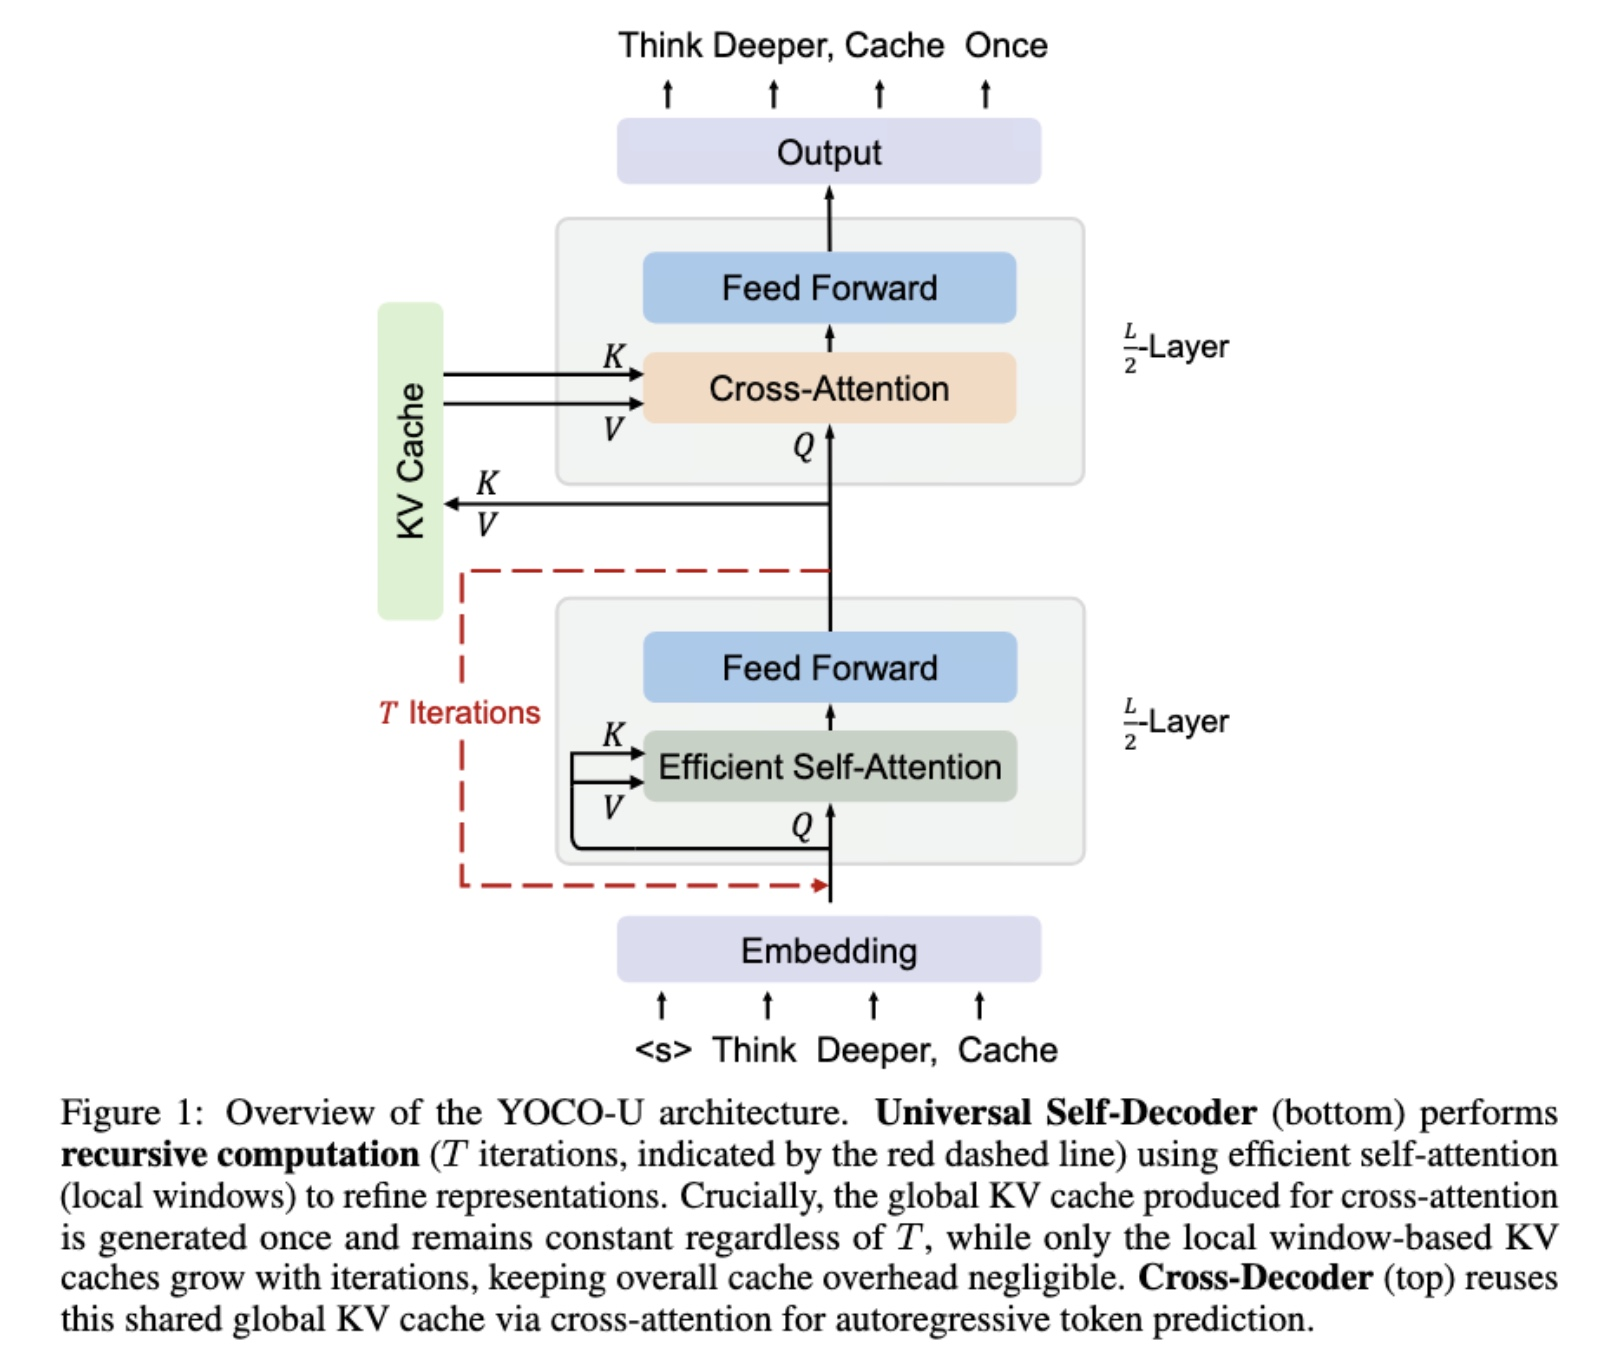
\includegraphics[width=0.65\linewidth,height=\textheight,keepaspectratio]{assets/YOCO-U_1.jpg}

\end{center}

YOCO-U 则是对前面的 Self-Decoder
上了今年一直疑云重重、热度一波接着一波来的 \textbf{Loop}：对前面的
Self-Decoder loop 三次后产生一份 Shared KV；在 Cross-Decoder
上的改动则是采用了 \textbf{NOPE}。

\begin{center}

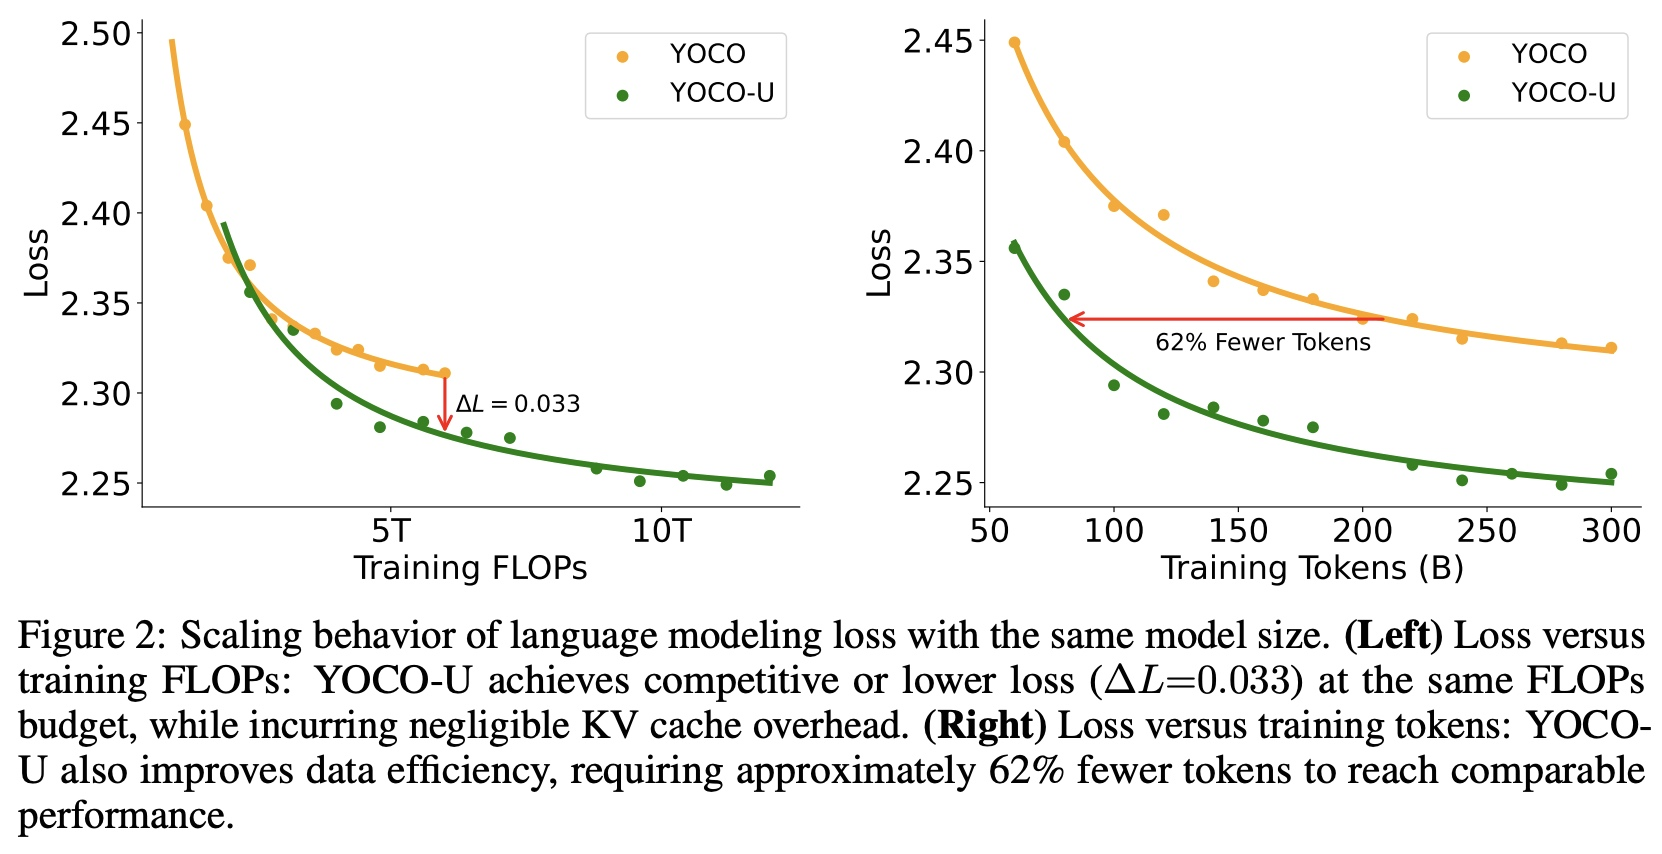
\includegraphics[width=0.75\linewidth,height=\textheight,keepaspectratio]{assets/YOCO-U_2.jpg}

\end{center}

\begin{center}

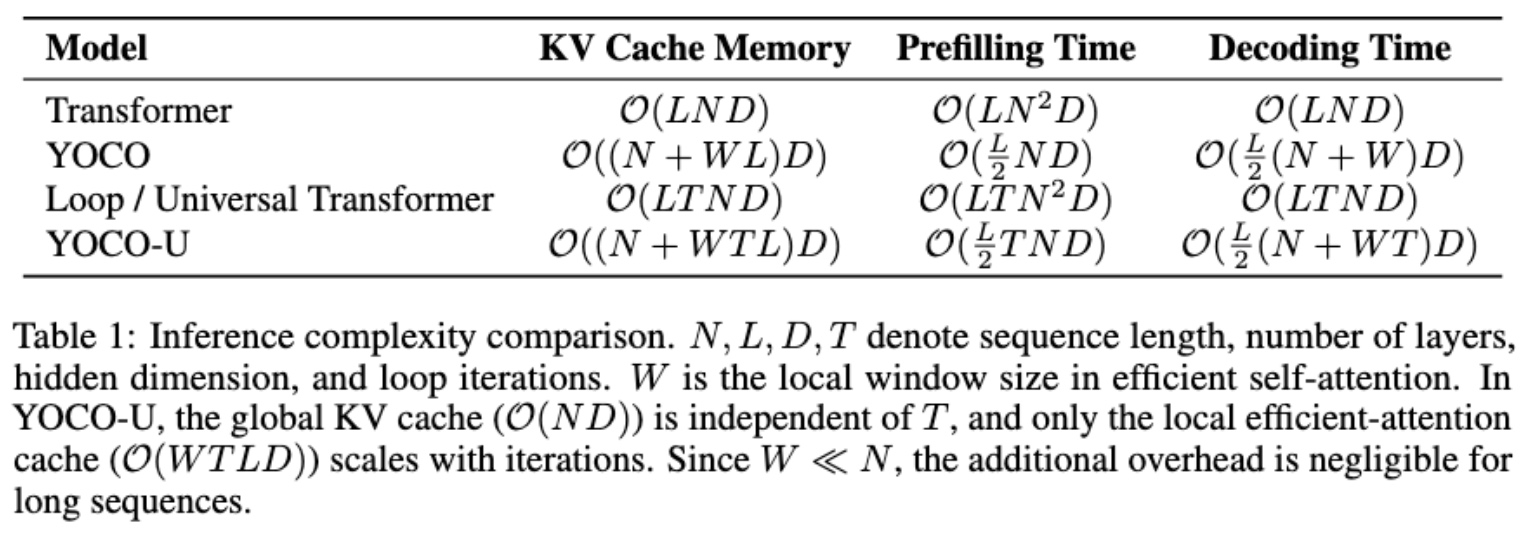
\includegraphics[width=0.8\linewidth,height=\textheight,keepaspectratio]{assets/YOCO-U_3.jpg}

\end{center}

\subsection{三、YOCO-Sparse}\label{ux4e09yoco-sparse}

\begin{center}

\pandocbounded{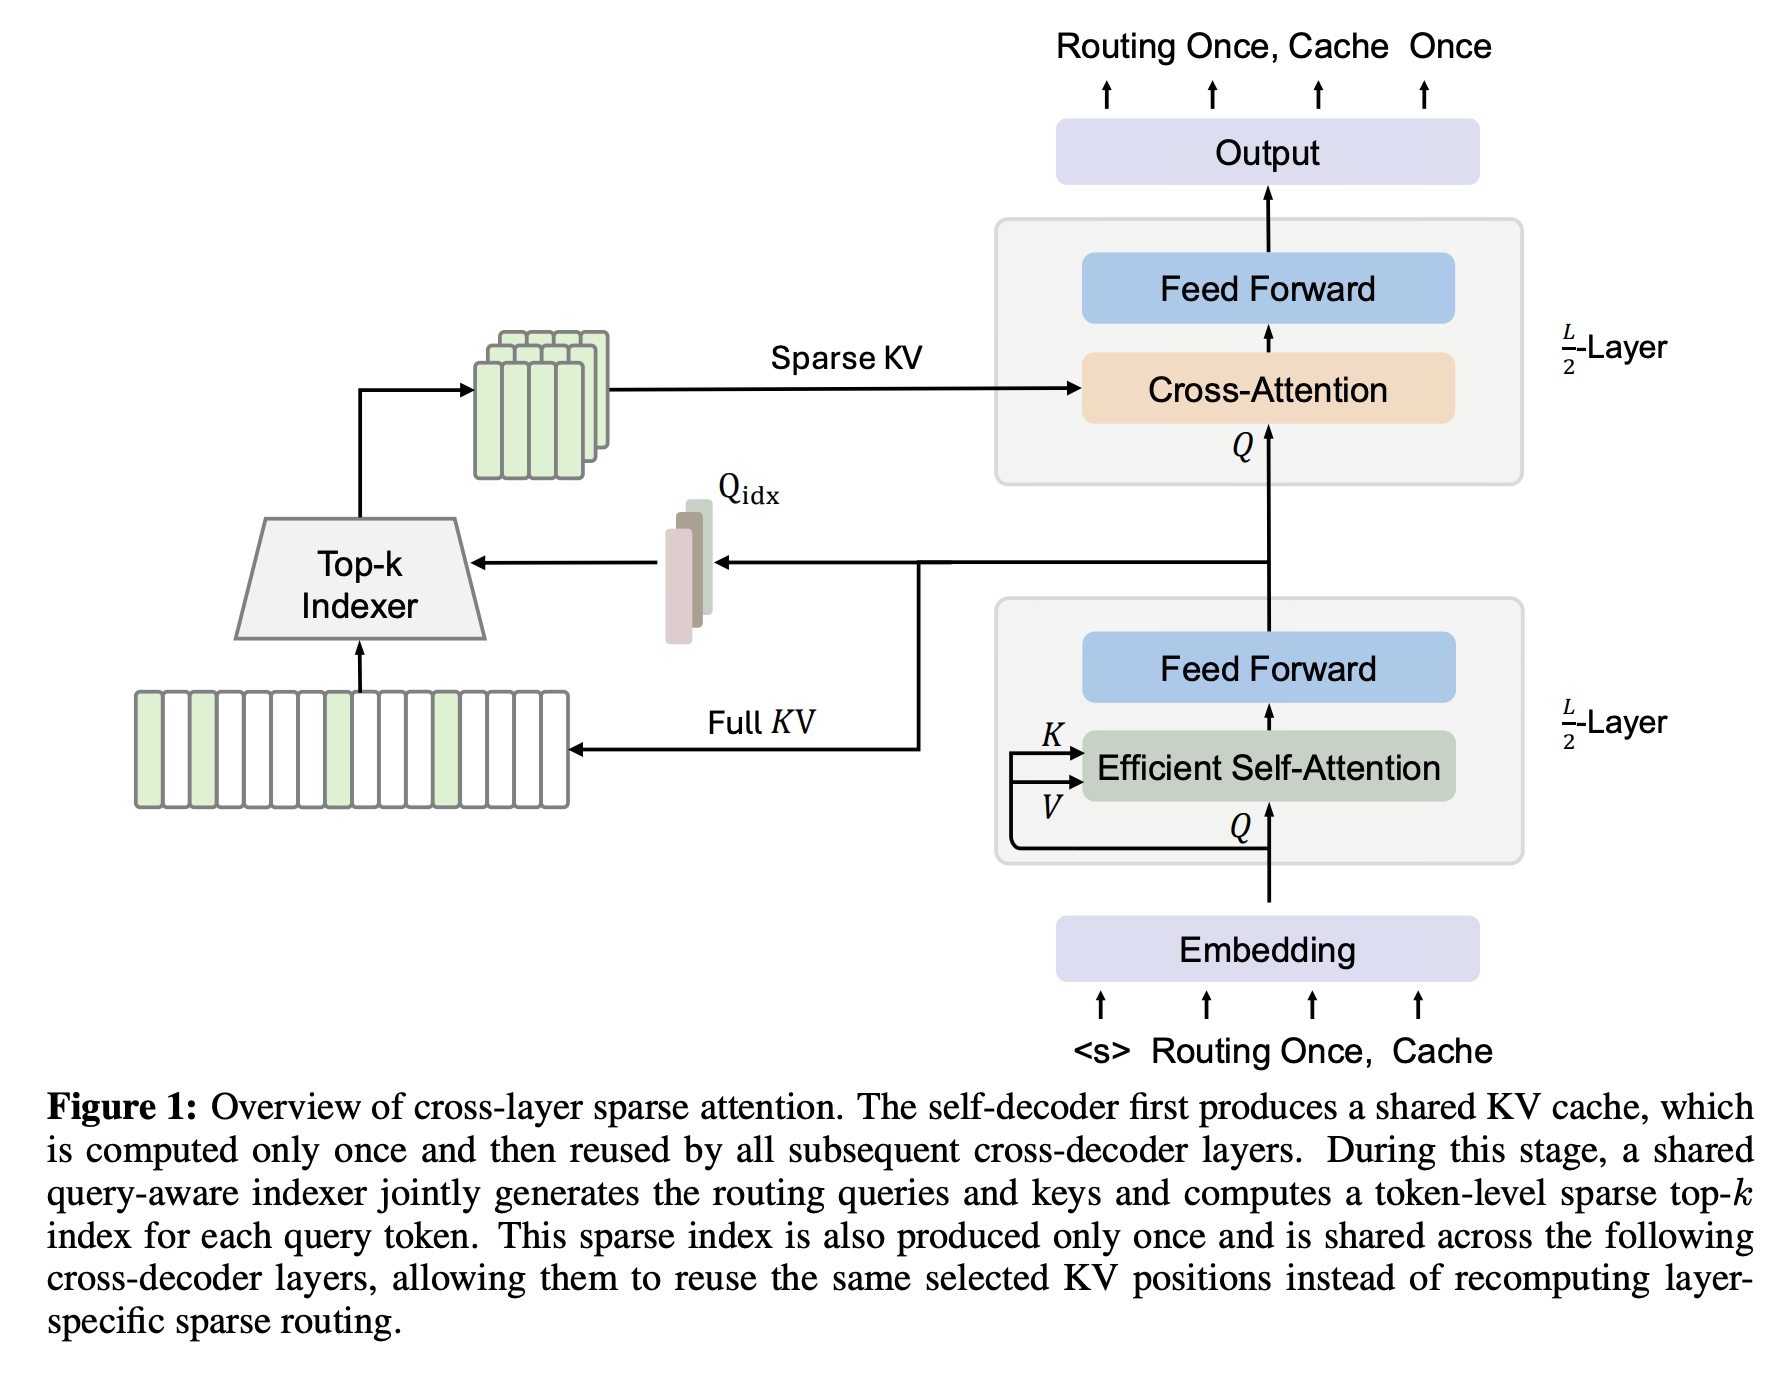
\includegraphics[keepaspectratio]{assets/YOCO-Sparse_1.jpg}}

\end{center}

YOCO-Sparse 的想法就更加干脆直接啦：既然 YOCO 后半部分的多个
Cross-Decoder layer 本来就在读取同一份 KV Cache，那干脆 \textbf{Sparse
Attention 的 Routing Index 也共享}得了，堪称省中省。

\begin{center}

\pandocbounded{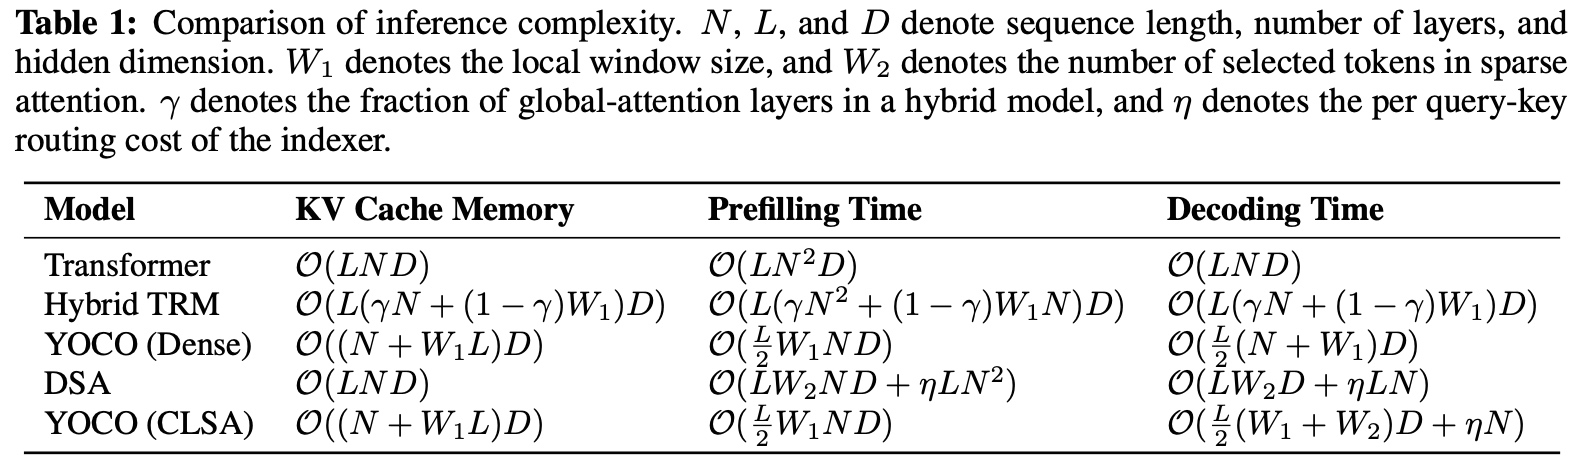
\includegraphics[keepaspectratio]{assets/YOCO-Sparse_2.jpg}}

\end{center}

\begin{center}

\pandocbounded{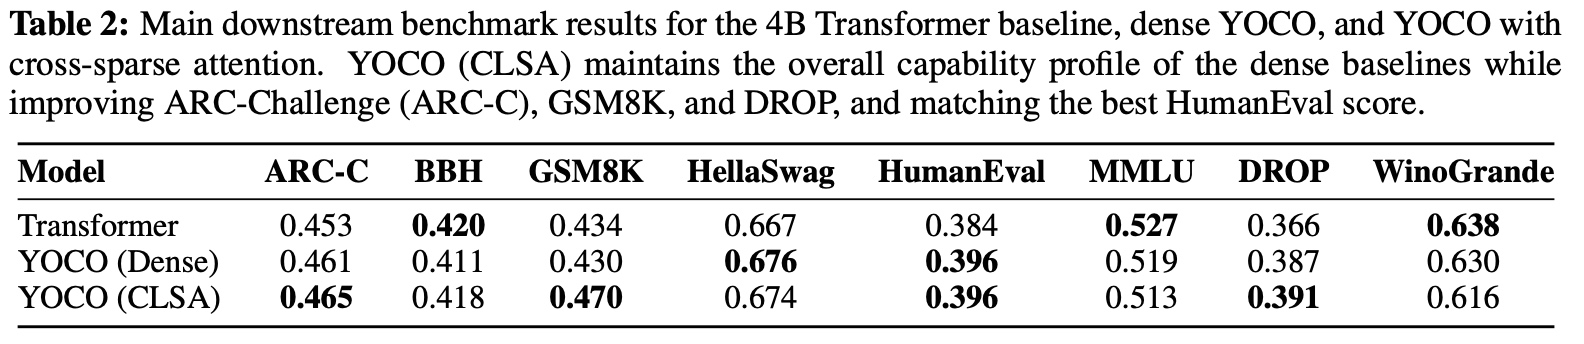
\includegraphics[keepaspectratio]{assets/YOCO-Sparse_3.jpg}}

\end{center}

\subsection{四、DeepSeek-V4.1-Flash}\label{ux56dbdeepseek-v4.1-flash}

\begin{center}

\pandocbounded{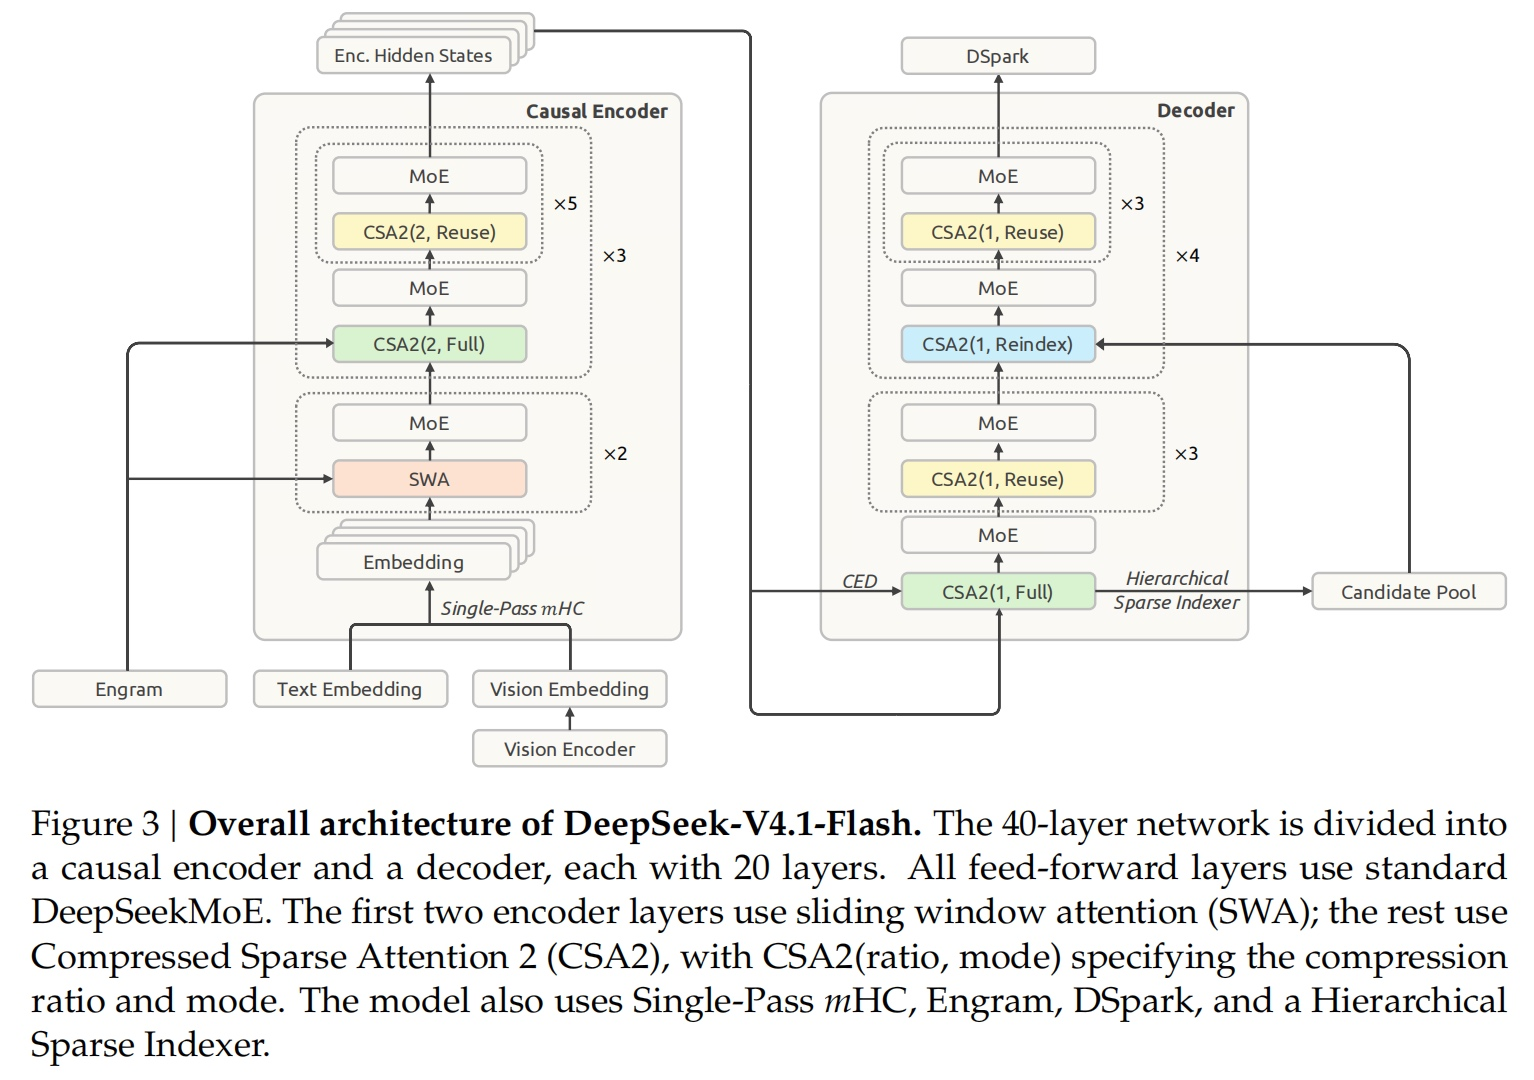
\includegraphics[keepaspectratio]{assets/DeepSeek-V4.1-Flash_1.jpg}}

\end{center}

DS 家一向是在压 KV 上最最最激进的，这次 4.1 更是令人``触目惊心''。

\begin{center}

\pandocbounded{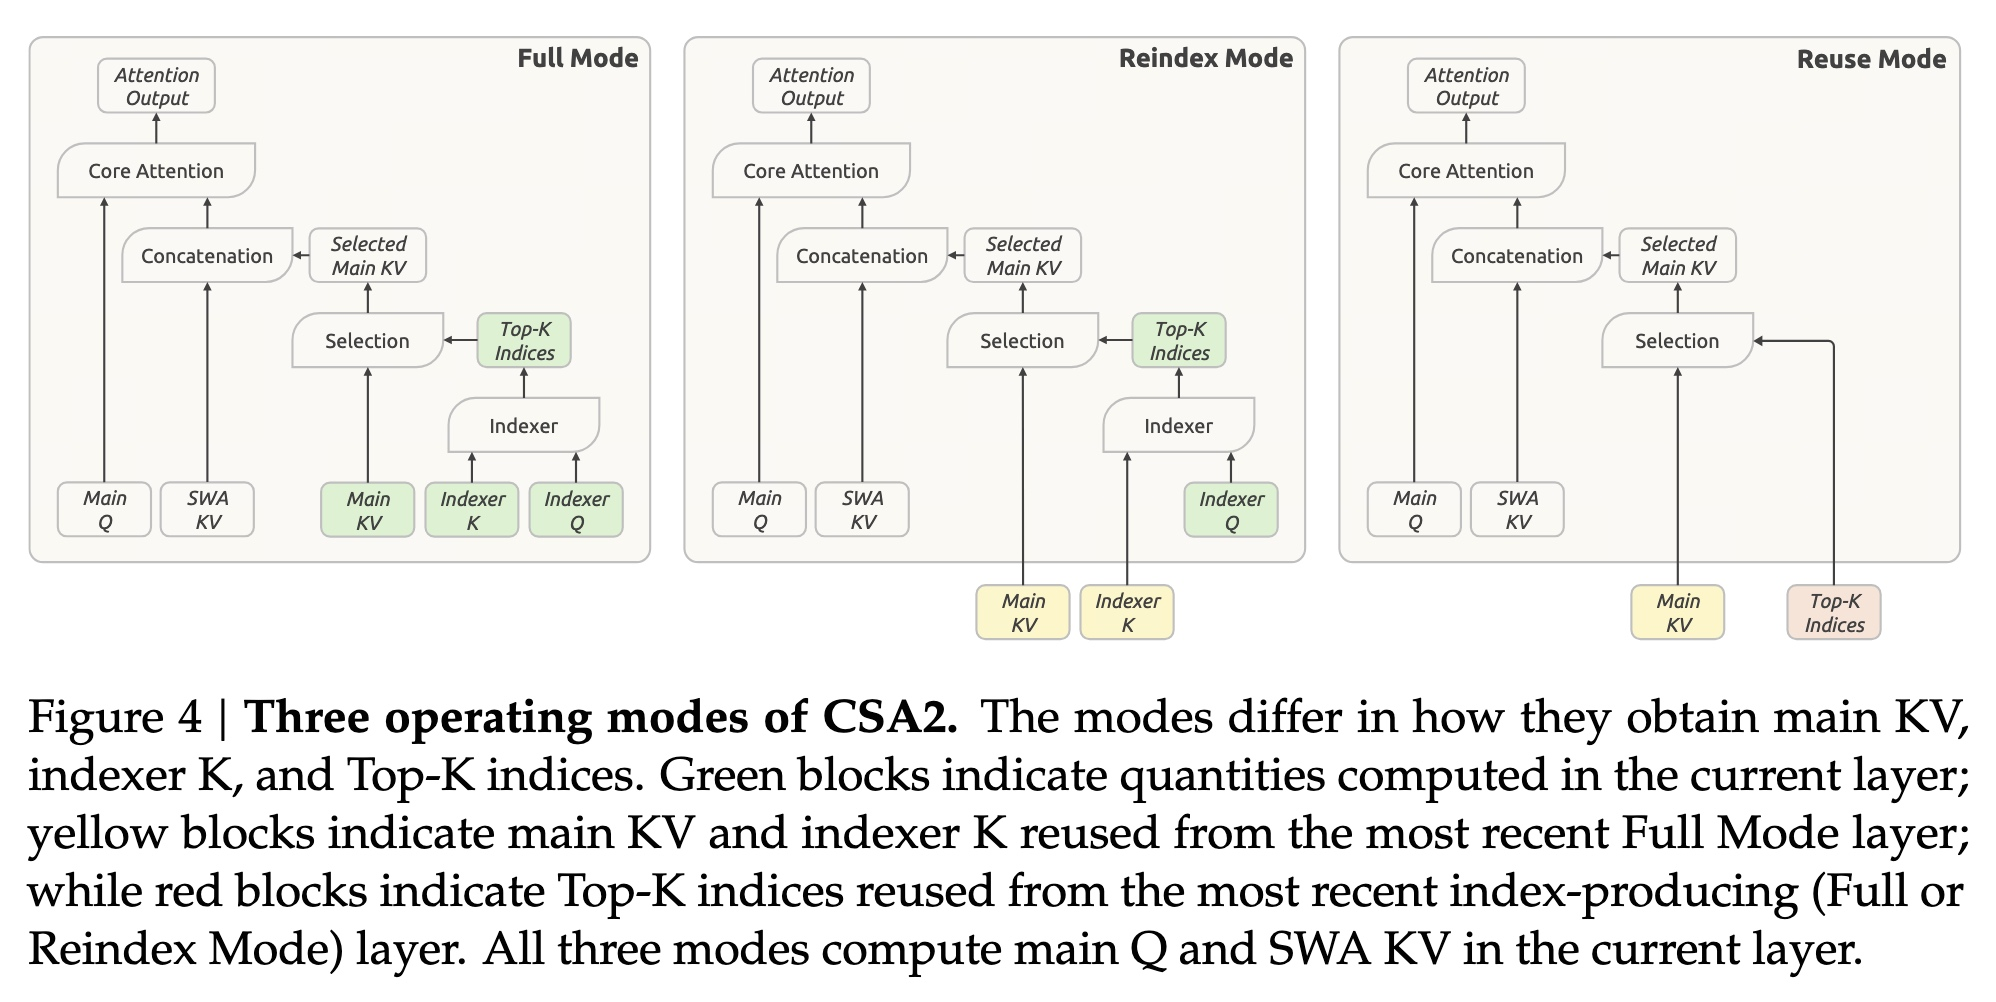
\includegraphics[keepaspectratio]{assets/DeepSeek-V4.1-Flash_2.jpg}}

\end{center}

DeepSeek-V4.1-Flash 的 Attention 大致为 \textbf{YOCO/CED + CSA2 + SWA}。

\subsubsection{YOCO/CED：减少 Prefill
计算}\label{yococedux51cfux5c11-prefill-ux8ba1ux7b97}

Global KV 以 YOCO 为大框架，把 40 层分成 \textbf{20 层 Causal Encoder +
20 层 Decoder}。 DS自己称之为 CED 架构。

在 Prefill 时跑前 20 层，Decoder 的 Global KV 直接由 Encoder 最后一层
\(H_{20}\) 通过各层独立投影生成，因此避免让整个 Prompt 再完整跑后 20
层。

\subsubsection{CSA2：跨层复用 Global KV 与
Top-K}\label{csa2ux8de8ux5c42ux590dux7528-global-kv-ux4e0e-top-k}

在此基础上，Global Attention 用 CSA2 做跨层复用：

\begin{itemize}
\tightlist
\item
  \textbf{Full 层}：生成新的 Global KV 和 Top-K。
\item
  \textbf{Reindex 层}：复用 KV，但重新选 Top-K。
\item
  \textbf{Reuse 层}：连 KV 和 Top-K 都复用。
\end{itemize}

Decoder 中只有第一个 Full 层生成 Global KV，后续层共享这份
KV，并每隔几层通过 Reindex 更新检索位置。Global Sparse Attention
最终只读取 \textbf{Top-512 个远程 KV}。

\subsubsection{SWA：短期缓存与局部重建}\label{swaux77edux671fux7f13ux5b58ux4e0eux5c40ux90e8ux91cdux5efa}

为了进一步省存储，DeepSeek 不再把 SWA KV 长期放进 persistent
cache：长期保存的主要是 Global KV，而 SWA KV 只放在短 TTL 的 host-DRAM
pool 中；\textbf{Global Main KV 使用 FP4，SWA KV 保留 FP8}。

如果 SWA KV 丢失，正常来讲，由于多层 SWA
的有效感受野会随着层数成倍扩大，重建 SWA 得 replay
\(128\times\text{layers}\) 个 token。但是 DS V4.1 直接只 \textbf{replay
最后 128 个 token}（他真的太能省了，我哭死\ldots\ldots）。

Decode 时，新 token 仍正常经过全部 40 层，并同时使用 \textbf{Top-512
Global Sparse KV + 128 Local SWA KV}。

\clearpage

\subsection{五、Gemma 4 E2B / E4B}\label{ux4e94gemma-4-e2b-e4b}

Gemma 4 其实在架构上有不少花活，而在 E2B / E4B 上也用了类似 YOCO
的技术。

说来也十分简单干脆：\textbf{后半段很多层不再计算自己的 K/V，只保留独立的
Q，并复用前面最后一个同类型 Attention 层的 KV。}

{\def\LTcaptype{none} % do not increment counter
\begin{longtable}[]{@{}
  >{\raggedright\arraybackslash}p{(\linewidth - 8\tabcolsep) * \real{0.2000}}
  >{\raggedright\arraybackslash}p{(\linewidth - 8\tabcolsep) * \real{0.2000}}
  >{\raggedright\arraybackslash}p{(\linewidth - 8\tabcolsep) * \real{0.2000}}
  >{\raggedright\arraybackslash}p{(\linewidth - 8\tabcolsep) * \real{0.2000}}
  >{\raggedright\arraybackslash}p{(\linewidth - 8\tabcolsep) * \real{0.2000}}@{}}
\toprule\noalign{}
\begin{minipage}[b]{\linewidth}\raggedright
模型
\end{minipage} & \begin{minipage}[b]{\linewidth}\raggedright
总层数
\end{minipage} & \begin{minipage}[b]{\linewidth}\raggedright
后段共享范围
\end{minipage} & \begin{minipage}[b]{\linewidth}\raggedright
Sliding Attention 复用来源
\end{minipage} & \begin{minipage}[b]{\linewidth}\raggedright
Full / Global Attention 复用来源
\end{minipage} \\
\midrule\noalign{}
\endhead
\bottomrule\noalign{}
\endlastfoot
\textbf{Gemma 4 E2B} & 35 层 & L15--L34 & L13 的 KV & L14 的 KV \\
\textbf{Gemma 4 E4B} & 42 层 & L24--L41 & L22 的 KV & L23 的 KV \\
\end{longtable}
}

\subsection{六、WeLM}\label{ux516dwelm}

WeLM 也做了类似 YOCO 的操作 \textbf{KV-Mirror}，但是本质目的不是为了节省
KV Cache，而是为了\textbf{节省 Prefill 的计算}。

具体而言，他们采用 \textbf{U 形的 KV 共享策略}：前 1/3 的层镜像到后 1/3
共享，并且是复用被镜像层在 \textbf{K/V 投影前的 Hidden States（而不是
KV！）}，再用目标层的投影重新计算 K/V，也就节省了 Prefill 阶段后 1/3
层的完整 Attention 和 MoE 等计算。

至于为什么是 U 形呢？是之前有篇文章 KVSharer
发现，\textbf{共享差异更大的 layer KV，性能反而更好}。

\end{document}
